\documentclass[bachelor, och, referat]{SCWorks}
% параметр - тип обучения - одно из значений:
%    spec     - специальность
%    bachelor - бакалавриат (по умолчанию)
%    master   - магистратура
% параметр - форма обучения - одно из значений:
%    och   - очное (по умолчанию)
%    zaoch - заочное
% параметр - тип работы - одно из значений:
%    referat    - реферат
%    coursework - курсовая работа (по умолчанию)
%    diploma    - дипломная работа
%    pract      - отчет по практике
%    pract      - отчет о научно-исследовательской работе
%    autoref    - автореферат выпускной работы
%    assignment - задание на выпускную квалификационную работу
%    review     - отзыв руководителя
%    critique   - рецензия на выпускную работу
% параметр - включение шрифта
%    times    - включение шрифта Times New Roman (если установлен)
%               по умолчанию выключен 

\usepackage[T2A]{fontenc}
\usepackage[utf8]{inputenc}
\usepackage{graphicx}
\usepackage[sort,compress]{cite}
\usepackage{amsmath}
\usepackage{amssymb}
\usepackage{amsthm}
\usepackage{fancyvrb}
\usepackage{longtable}
\usepackage{array}
\usepackage{makecell}
\usepackage{multirow}
\usepackage[english,russian]{babel}

\usepackage{tempora}
\usepackage[hidelinks]{hyperref}

\usepackage{pgfplots}
\usepackage{tikz}
\usepackage{float}
\pgfplotsset{compat = newest}

% \usepackage{minted}
% \setminted[c++]{linenos, breaklines = true, style = bw, fontsize = \small}


\newcommand{\eqdef}{\stackrel {\rm def}{=}}

\newtheorem{lem}{Лемма}

\begin{document}


% Кафедра (в родительном падеже)
%\chair{математической кибернетики и компьютерных наук}

% Тема работы
\title{Готовые лабораторные работы по физике 2 семестр 1 курс.}

% Курс
\course{1}

% Группа
\group{151}

% Факультет (в родительном падеже) (по умолчанию "факультета КНиИТ")
%\department{факультета КНиИТ}

% Специальность/направление код - наименование

\napravlenie{09.03.04 "--- Программная инженерия}

% Фамилия, имя, отчество в родительном падеже
\author{Смирнова Егора Ильича}

% Год выполнения отчета
\date{2024}

\maketitle

% Включение нумерации рисунков, формул и таблиц по разделам
% (по умолчанию - нумерация сквозная)
% (допускается оба вида нумерации)
%\secNumbering

\tableofcontents

% Раздел "Обозначения и сокращения". Может отсутствовать в работе
%\abbreviations
%\begin{description}
%    \item $|A|$  "--- количество элементов в конечном множестве $A$;
%    \item $\det B$  "--- определитель матрицы $B$;
%    \item ИНС "--- Искусственная нейронная сеть;
%    \item FANN "--- Feedforward Artifitial Neural Network
%\end{description}

% Раздел "Определения". Может отсутствовать в работе
%\definitions

% Раздел "Определения, обозначения и сокращения". Может отсутствовать в работе.
% Если присутствует, то заменяет собой разделы "Обозначения и сокращения" и "Определения"
%\defabbr


% Раздел "Введение"
\intro

Здесь вы можете найти готовые лабораторные работы за 2 семестр 1 курса, которые мы выполняли. Возможно вам придется что"=то переделать, но мне кажется пофиксить пару моментов в готовом сильно проще, чем хуярить с нуля (Делать одну сраную лабу 1.5 месяца очень весело, надеюсь вас это не настигнет).

\section{Лабораторная работа <<Поверхностное натяжение>>}

\textbf{Цель работы:} определение коэффициента поверхностного натяжения методом <<Разрыва тонкого слоя жидкости>>.

\textbf{Принадлежности:} кольцо для изучения поврхностного натяжения, точный динамометр $(0.1H)$, стакан из комплекта дополнительного оборудования, лабораторный подъёмный столик со штативом из нержавеющей стали и крючком, штангенциркуль.Установка (рис.\ref{fig:installation})

\begin{figure}[!h]
    \centering
    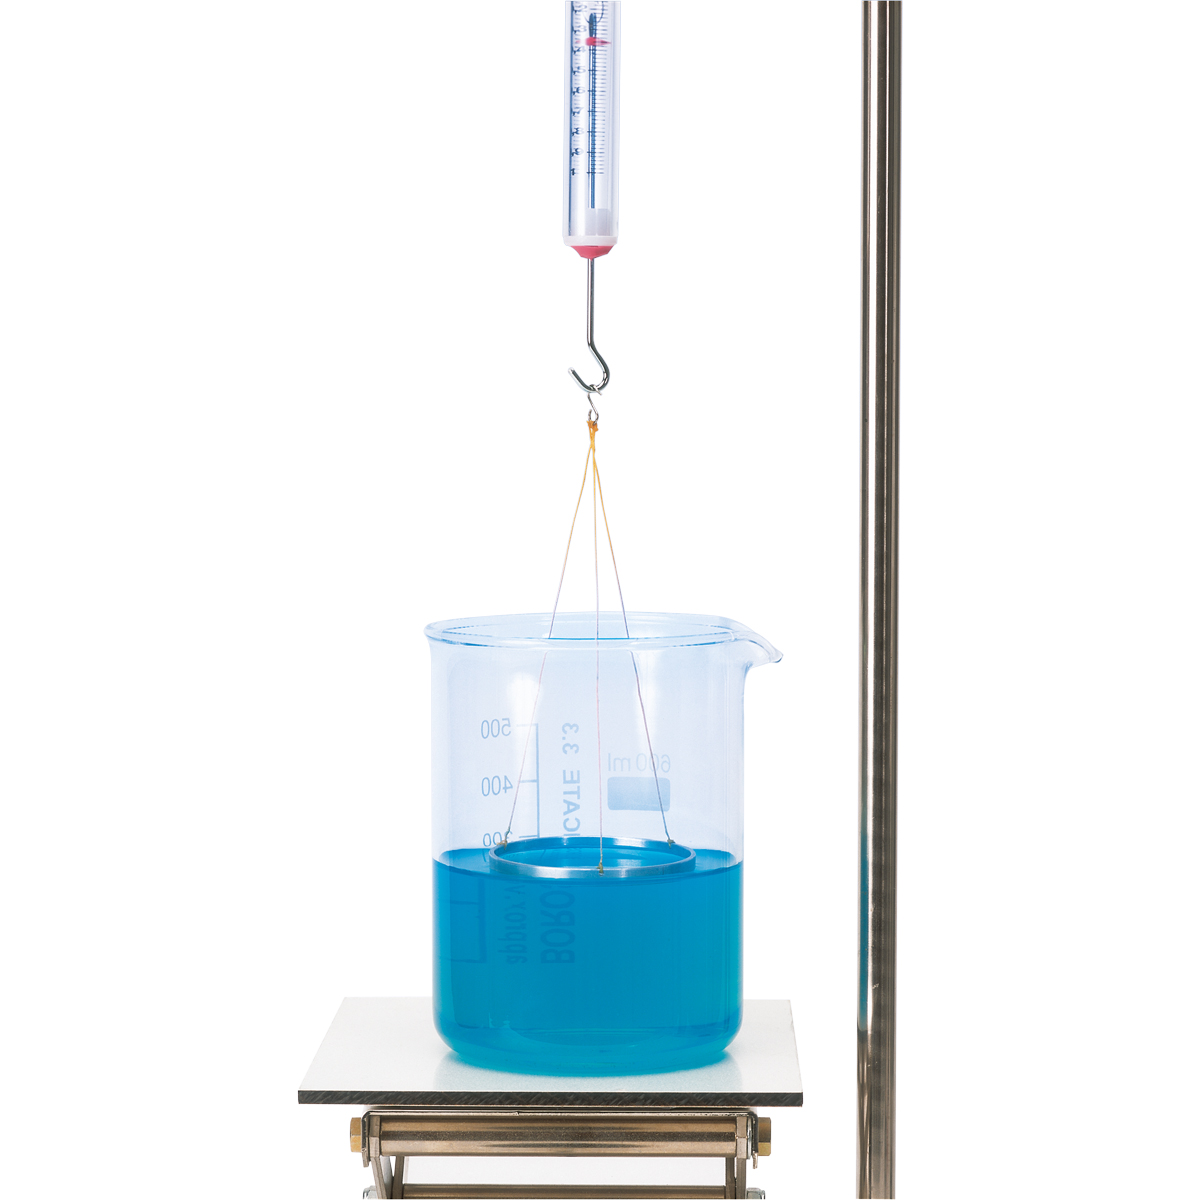
\includegraphics[width = 0.5\textwidth]{image/image.png}
    \caption{установка}
    \label{fig:installation}
\end{figure}

\textbf{Вывод рабочей формулы:}

Поверхностное натяжение жидкости "--- это её свойство на границе контакта с окружающей средой. Оно обусловлено тем, что молекула жидкости, находящаяся на её поверхности, испытывает действие сил со стороны соседних с ней молекул жидкости только из половины пространства, ограниченной поверхностью этой жидкости, в то время как молекула внутри жидкости испытывает воздействие со всех сторон. Поэтому молекула в поверхностном слое испытывает воздействие результирующей силы, направленной перпендикулярно к поверхности внутрь жидкости.

Действие этой силы приводит к сокращению площади поверхности жидкости. Взаимодействие молекул в поверхностном слое также обуславливает наличие горизонтальной составляющей сил, способствующей стремлению площади поверхности к сокращению. Эти силы получили название сил поверхностного натяжения. Сила поверхностного $F_\text{н}$ натяжения направлена по касательной к поверхности жидкости. За счёт воздействия сил поверхностного натяжения молекулы жидкости в поверхностном слое обладаююь дополнительной потенциальной энергией по сравнению с молекулами внутреннего объема. Это дополнительная энергия называется поверхностной энергией $W_\text{пов}$ и пропорциональна площади поверхности жидкости:

\begin{equation*}
    W_\text{пов} = \alpha S
\end{equation*}

Коэффициент пропорциональности $\alpha$ является мерой свободной поверхности.

\begin{equation*}
    \alpha = \frac{W_\text{пов}}{S}
\end{equation*}

называется коэффициентом поврхностного натяжения и зависит от природы и состояния как жидкости, так и той среды с которой соприкасается её поверхность. То есть от физико"=химических свойств, определяющих энергию взаимодействия их молекул.

Физический смысл коэффициента поверхностного натяжения состоит в том, что он численно равен рабооте, затрачиваемой на образование $1 \text{м}^2$ поверхности жидкости при постоянной температуре.

\begin{equation*}
    \alpha = \frac{d A_\text{пов}}{d S}
\end{equation*}

и представляет собой силу сцепления поверхностной плёнки жидкости. Вызванную взаимным притяжением молекул, находящихся по обе стороны линии контура её разрыва, дейстующую на единицу длины:

\begin{equation*}
    F_\text{н} = \alpha L
\end{equation*}

Определить коэффициент поверхностного натяжения можно увеличив поверхность жидкости на величин $d S$ переводом в поверхностный слой некоторого числа молекул, совершив тем самым работы $d A_\text{пов}$. Осуществить это возможно при помощи кольца с острой кромкой, которое изначально полностью погружено в жидкость. Если, приложив внешнюю силу $F_\text{вн}$, компенсирующую силу поверхностного натяжения $F_\text{вн}$, кольцо медленно извлеать из жидкости, тонкий слой жидкости вытягивается вверх за его нижним краем (рис. \ref{fig:installation})

\begin{equation*}
    d A_\text{пов} = F_\text{вн} \Delta x
\end{equation*}

Когда кольцо поднимается на высоту $\Delta x$, площадь поверхности тонкого слоя увеличивается снаружи и внутри кольца в общем на:

\begin{equation*}
    d S = 4 \pi R \Delta x
\end{equation*}

где $R$ "--- радиус кольца. 

Если сила $F_\text{вн}$, прилагаемая при подъёме кольца, превышает $F_\text{н}$, тонкий слой жидкости рвется. В этот момент можно определить:

\begin{equation}
    \alpha = \frac{F_\text{вн}}{4 \pi R}
    \label{eq : alpha}
\end{equation}

\vspace{0.5cm}

\textbf{Описание установки:}

В этой работе металлическое кольцо с острой нижней кромкой свисает в горизонтальном положении с точного динамометра. Сначала кольцо полностью погружено в испытываемую жидкость (например, в воду), затем оно медленно извлекается из жидкости. Тонкий слой жидкости разрывается, когда сила вытягивания $F_\text{вн}$, превышает предельное значение $F_\text{н}$.

\vspace{0.5cm}

\textbf{Порядок выполнения работы:}
\begin{enumerate}
    \item {Установить лабораторный подъёмный столик на минимальный уровень подъёма.}
    \item {Подвесить динамометр на вертикальный штатив с крючком.}
    \item {Измерить диаметр кольца и подвесить его к динамометру.Значения диаметра занести в таблицу.}
    \item {Наполнить стакан исследуемой жидкостью и поставить его на лабораторный подъёмный столик.}
    \item {Поднять стакан подъёмным столиком до погружения в жидкость острой нижней кромки кольца.}
    \item {Записать показание динамометра $F_1$ в таблицу}
    \item {Медленно опустить лабораторный подъёмный столик со стаканом до момента разрыва пленки (отрыва кольца от жидкости).}
    \item {В момент разрыва снять показание динамометра $F_2$ и занесите в таблицу}
    \item {
        Рассчитать и занести в таблицу \ref{tab:my_label} разницу между двумя значениями силы:
        \begin{equation*}
            F_\text{вн} = F_2 - F_1
        \end{equation*}
    }
    \item {Повторить измерение несколько раз и проверить воспроизводимость.}
    \item {Используя полученные данные, вычислить по формуле \ref{eq : alpha} значение коэффициента поверхностного натяжения $\alpha$ исследуемой жидкости для каждого измерения и занести в таблицу}
    \item {Определить среднее значение коэффициента поверхностного натяжения $\alpha _\text{ср}$, абсолютною погрешность $\Delta \alpha$ и среднее значение абсолюной погрешности $\Delta \alpha _\text{ср}$.Занести полученные данные в таблицу \ref{tab:my_label} (Значение коэфициента поверхностного натяжения эталонной жидкости $\Delta \alpha _\text{табл}$ для расчетов взять из справочных данных.)}
    \item {Записать полученный результат в таблицу $\alpha _\text{ср} \pm \Delta \alpha _\text{ср}$.}
    \item {
        Вычислить относительную погрешность измерений {$\delta$} по формуле:
        \begin{equation*}
            \delta = \frac{\delta \alpha _ \text{ср}}{\alpha _ \text{ср}} \cdot 100\% 
        \end{equation*}
    }
    \item {
        Сравнить полученное значение коэффициента поверхностного натяжения с его табличным значением. Сравнить расхождение экспериментально полученного и табличного значений по формуле:
        \begin{equation*}
            \Delta \sum =  \left(\frac{| \alpha _\text{ср} - \alpha _\text{табл}|}{\alpha _\text{табл}} \right) \cdot 100\%
        \end{equation*}
    }
\end{enumerate}
    
\[\ln{\alpha}=\ln{F_{vn}} - \ln{4\pi} - \ln{R}\]\
\[d\alpha= d F_{vn} - d R\]

\[|\frac{\Delta \alpha}{\alpha}| = |\frac{\Delta F_{vn}}{F_{vn}}| + |\frac{\Delta R}{R}|\]

\[|\frac{\Delta \alpha}{\alpha}| = (|\frac{0,001}{0,02}| + |\frac{1}{30}|) \cdot 100 \% = (|\frac{1}{20}| + |\frac{1}{30}|) \cdot 100 \% = 8,3 \%\]

\begin{table}[!h]
    \centering
    \resizebox{\textwidth}{!}{
    \begin{tabular}{|c|c|c|c|c|c|c|c|c|c|c|c|c|}
         \hline
         %первая часть превой строки
         \makecell{№\\опы\\та} &
         \makecell{Диам\\етр\\коль\\ца\\$D_\text{к}$,м}&
         \multicolumn{2}{|c|}{\makecell{Пока\\зания\\динамо\\метра}}&
         \makecell{Дейст\\вую\\щая\\сила\\$F_\text{вн}$, H}&
         \multicolumn{3}{|c|}{\makecell{Коэффициэнт\\поверхностного\\натяжения}}&
         \multicolumn{3}{|c|}{\makecell{Погрешность\\изменения}}&
        \makecell{Полу\\ченный\\резуль\\тат\\$\alpha _\text{ср} \pm$\\$ \Delta \alpha _\text{ср}$} &
         \makecell{Расхож\\дение с\\таблич\\ным зна\\чением\\$\Delta \sum $,$ \%$}\\
         %вторая часть первой строки
         \cline{3-4}\cline{6-8}\cline{9-11}
         & & \makecell{$F_1 $,\\H}& \makecell{$F_2 $,\\H}& &
         \makecell{Изме\\рен\\ный\\$\alpha $,$\frac{H}{\text{м}}$}&
         \makecell{Сред\\нее\\$\alpha _\text{ср}$,\\$\frac{H}{\text{м}}$}&
         \makecell{Таб\\лич\\ный\\$\alpha _\text{табл}$,\\$\frac{H}{\text{м}}$}&
         \makecell{Абсо\\лют\\ная\\$\Delta \alpha$,\\$\frac{H}{\text{м}}$}&
         \makecell{Сред\\нее\\$\Delta \alpha _\text{ср}$,\\$\frac{H}{\text{м}}$}&
         \makecell{Отно\\ситель\\ная\\$\delta$,$\%$}& &\\
         \hline
         1& & \makecell{0.051}& \makecell{0.072}& \makecell{0.021}& \makecell{0.056}& & & \makecell{0.015}& & & & & 
         \cline{1-1}\cline{3-6}\cline{9-9}
         2& & \makecell{0.052}& \makecell{0.073}& \makecell{0.021}& \makecell{0.056}& & & \makecell{0.015}& & & & &
         \cline{1-1}\cline{3-6}\cline{9-9}
         
         3& \makecell{0.06}& \makecell{0.051}& \makecell{0.073}& \makecell{0.022}& \makecell{0.058}& \makecell{0.055}& \makecell{0.071}& \makecell{0.013}& \makecell{0.0158}& \makecell{1.81}& \makecell{0.055\\$\pm$\\0.0158}& \makecell{22.53}&
         
         \cline{1-1}\cline{3-6}\cline{9-9}
         4& & \makecell{0.052}& \makecell{0.072}& \makecell{0.02}& \makecell{0.053}& & & \makecell{0.018}& & & & &
         \cline{1-1}\cline{3-6}\cline{9-9}
         5& & \makecell{0.052}& \makecell{0.072}& \makecell{0.02}& \makecell{0.053}& & & \makecell{0.018}& & & & &
         \hline
    \end{tabular}
    }
    \caption{Измерения}
    \label{tab:my_label}
\end{table}

\textbf{Вывод:}

Определили коэффициент поверхностного натяжения воды методом разрыва тонкого слоя жидкости. Нашли относительную погрешность коэффициента поверхностного натяжения воды и рассчитали расхождение с табличным значением коэффициента поверхностного натяжения.

Максимальная погрешность больше экпериментальной (\(8,3 \% > 1,81 \%\) ), что означает, что опыт проведён правильно.



\section{Лабораторная работа <<Закон Бойля-Мариотта>>}

\textbf{Цель работы:} Подтверждение закона Бойля-Мариотта.

\textbf{Оборудование:} Установка для демонстации закона Бойля-Мариотта (рис.\ref{fig:установка для демнострации закона Бойля-Мариотта})

\begin{figure}[!h]
    \centering
    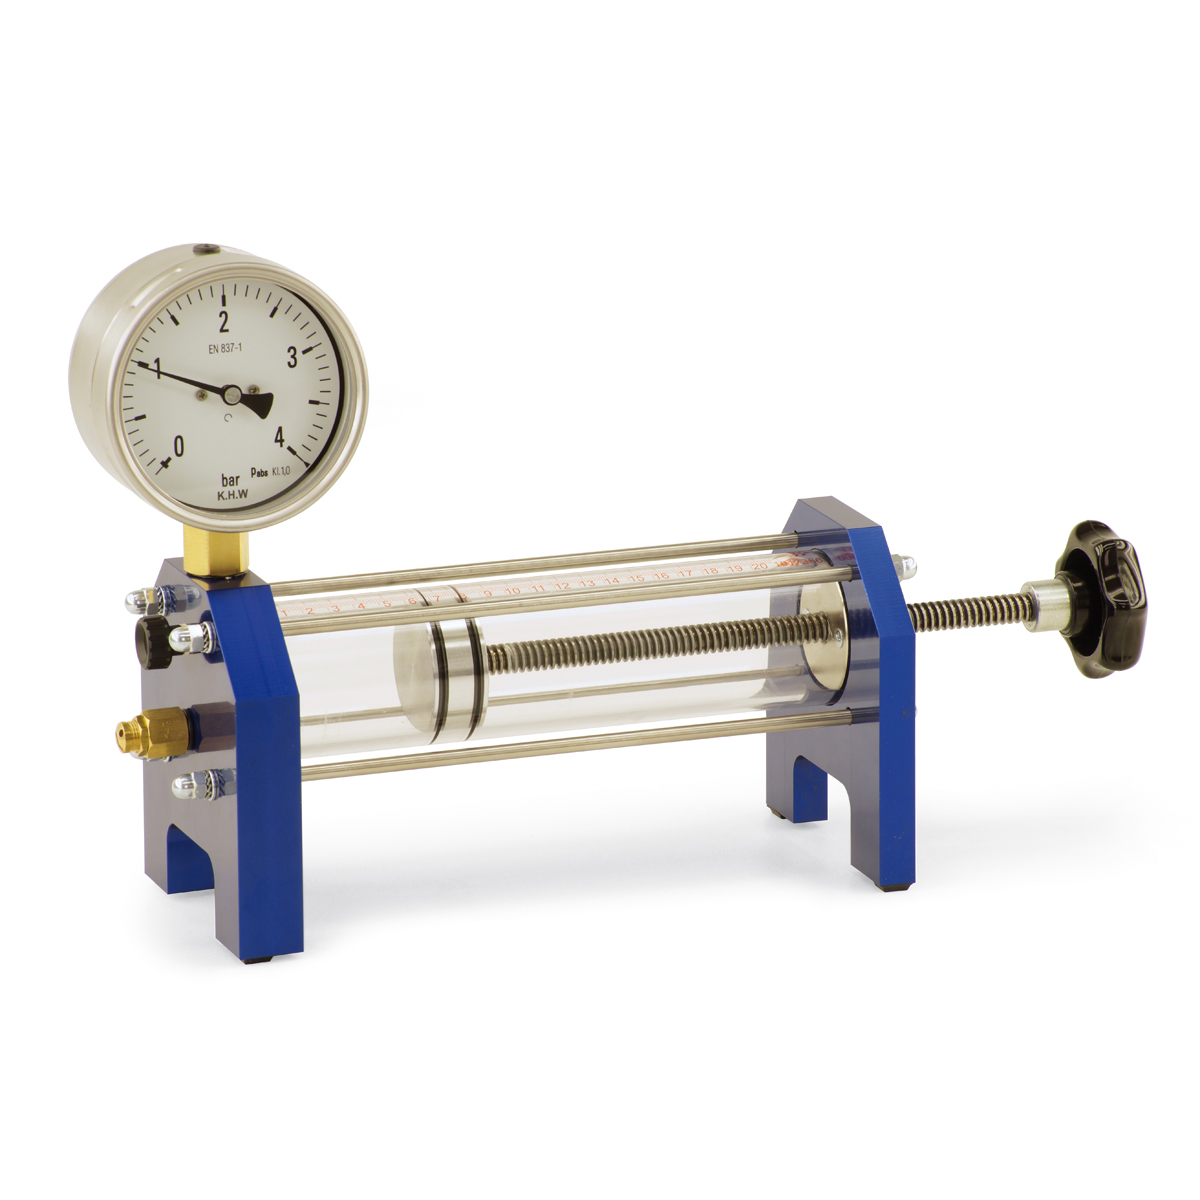
\includegraphics[width = 0.3\textwidth]{image/image2.png}
    
    \caption{Установка для демонстации закона Бойля-Мариотта}
    
    \label{fig:установка для демнострации закона Бойля-Мариотта}
\end{figure}

\textbf{Ход работы:}

\begin{enumerate}
    \item{Открыли запорный вентиль на левой опоре установки.}
    \item{Установили поршень внутри прозрачноо цилиндра в положение $S_0 = 20 ~ \text{см}$ и закрыли вентиль.}
    \item{Сняли показание давления и записли в таблицу \ref{tab:main_tab}.}
    \item{Изменяли положение поршня по 1"=му см. В каждом положении снимали и записывали показания давления в цилиндре}
    \item{Установили поршень в положение $S_0$, открыли вентиль, сбросив давление, и закрыли.}
    \item{Затем установили поршень в положение $S = 20$. Изменяли положение поршня пошагово по 1"=му см. В каждом положении снимали и регистрировали показания давления.}
    \item{Установили поршень в положение $S_0 = 5$, открыли вентиль сбросив давление, и закрыли.}
    \item{Затем установили поршень в положение $S = 20$. Изменяли положение поршня пошагово по 1"=му см. В каждом положении давления.}
    \item{Расчитали объем воздуха $V$, находящегося в закрытом пространстве цилиндра лаборатоной установки по данным о расстоянии $S$, на котором находится поршень по отношению к положению нулевого объема и площади поперечного сечения A поршня.}
    \item{Рассчитали при помощи уравнения $p V = \nu R T$, (где $T$ "--- температура газа, $R$ "--- универсальная газовая постоянная, $\nu$ "--- количество вещества) количество вещества в цилиндре, выраженное в молях}
    
    $
        \nu_1 = \frac{565.49}{8.314 \cdot 293.15} \approx 23.2 \text{мМоль}
    $
    
    $
        \nu_2 \approx 46.4 \text{мМоль}
    $
    
    $
        \nu_3 \approx 92.81 \text{мМоль}
    $
    \item{Построили графики зависимости $P$ от $V$ (рис.\ref{graph:main_graph})}
\end{enumerate}

\textbf{Эксперементальные данные:}

Эксперементальные данные представленны в таблице \ref{tab:main_tab}
\begin{table}[H]
    \centering
    \begin{tabular}{|c|c|c|c|c|}
        \hline
        \makecell{Положение \\ поршня $S$, см} & 
        \makecell{Рабочий объем \\ цилиндра $V \text{, см}^3$} &
        \multicolumn{3}{|c|}{\makecell{Давление воздуха при различном \\ его количестве в рабочем объеме \\ цилиндра $p$, бар}} \\
        \cline{3-5}
        & & {$S_0 = 20$} & {$S_0 = 10$} & {$S_0 = 5$}\\ 
        \hline 
        1 & 113.09 & - & - & 3 \\
        \hline 
        2 & 226.19 & - & 3.84 & 2.12 \\
        \hline 
        3 & 339.29 & - & 2.9 & 1.55 \\
        \hline 
        4 & 452.39 & - & 2.29 & 1.22 \\
        \hline 
        5 & 565.49 & 3.63 & 1.9 & 1 \\
        \hline 
        6 & 678.58 & 3.09 & 1.61 & 0.85 \\
        \hline 
        7 & 791.68 & 2.7 & 1.4 & 0.73 \\
        \hline 
        8 & 904.78 & 2.4 & 1.23 & 0.65 \\
        \hline 
        9 & 1017.9 & 2.15 & 1.1 & 0.58 \\
        \hline 
        10 & 1130.97 & 1.95 & 1 & 0.5 \\
        \hline 
        11 & 1244.1 & 1.79 & 0.91 & 0.47 \\
        \hline 
        12 & 1357.2 & 1.64 & 0.84 & 0.43 \\
        \hline 
        13 & 1470.3 & 1.51 & 0.78 & 0.4 \\
        \hline 
        14 & 1583.4 & 1.4 & 0.71 & 0.36 \\
        \hline 
        15 & 1696.5 & 1.31 & 0.67 & 0.35 \\
        \hline 
        16 & 1809.6 & 1.22 & 0.62 & 0.33 \\
        \hline 
        17 & 1922.7 & 1.18 & 0.59 & 0.3 \\
        \hline 
        18 & 2035.8 & 1.1 & 0.55 & 0.28 \\
        \hline 
        19 & 2148.8 & 1.05 & 0.52 & 0.26 \\
        \hline 
        20 & 2261.9 & 1 & 0.5 & 0.25 \\
        \hline
\end{tabular}
\caption{Эксперементальныйе данные}
\label{tab:main_tab}
\end{table}

Вывод:

В лабораторной работе мы проверили закон Бойля"=Мариотта, измерили давление воздуха при постоянном количестве вещества и температуре, передвигая поршень, и построили графики зависимости давления от объёма. Закон Бойля"=Мариотта действует, т.к. для всех измеренных значений $p V = const$ построенные графики гиперболические, что так же подтверждает закон

\begin{figure}[!h]
\begin{center}
\begin{tikzpicture}
    \begin{axis}
        [
            width=\linewidth, % Scale the plot to \linewidth 
            legend pos = north east,
            xlabel=$V ~ \text{см}^3$, % Set the labels
            ylabel=$p ~ \text{бар}$,
            ymin = 0,
            xmin = 0,
            grid = major
        ]
        \addplot table[x=column 1,y=column 2,col sep=comma] {csvTable/table1.csv}; 
        \addplot table[x=column 1,y=column 2,col sep=comma] {csvTable/table2.csv};
        \addplot table[x=column 1,y=column 2,col sep=comma] {csvTable/table3.csv};
        \legend{
            $S_0 = 20$,
            $S_0 = 10$,
            $S_0 = 5$,
        };
      \end{axis}
    \end{tikzpicture}
  \end{center}
\caption{График зависимости $P$ от $V$}
\label{graph:main_graph}
\end{figure}


\section{Лабораторная работа <<Определение отношения молярных теплоёмкостей газов адиабатическим методом>>}

\textbf{Принадлежности:} установка для определения отношения молярных теплоемкостей газа адиабатическим методом.

\begin{center}
    \textbf{Оборудование.}
\end{center}

Для проведения опыта служит прибор (рис. \ref{fig:установка 3.}), состоящий из большой стеклянной бутыли A, в горловину которой вставлена герметичная пробка. Через пробку проходит латунная трубка, имеющая два отвода: один a соединен с насосом, служащим для накачивания воздуха в сосуд, другой c – с манометром M. Сверху латунная трубка плотно закрывается резиновой пробкой в.

\begin{figure}[!h]
    \centering
    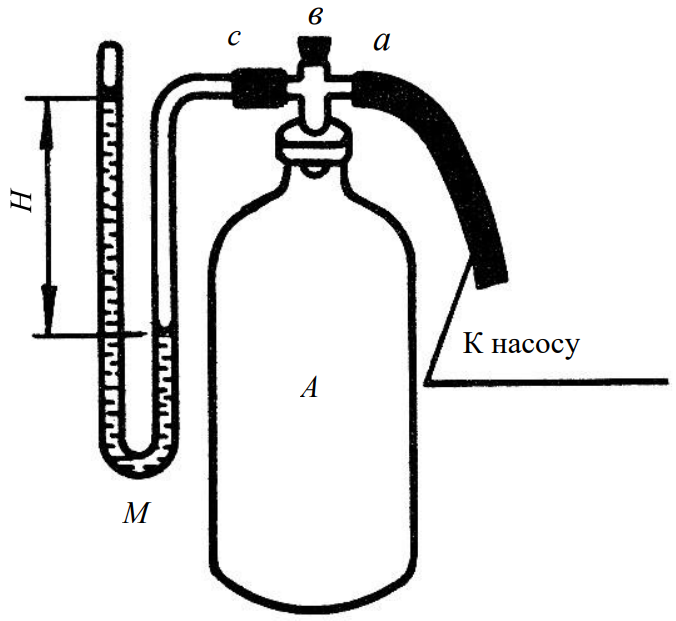
\includegraphics[width = 0.3\textwidth]{image/image3.png}
    
    \caption{Установка для Определения отношения молярных теплоемкостей газа адиабатическим методом.}
    
    \label{fig:установка 3.}
\end{figure}

Отношение количества теплоты $dQ$, сообщенного системе (телу), к соответствующему повышению температуры $dT$ называют теплоёмкостью:

\begin{equation}
    C_\text{тела} = \frac{d Q}{d T}
    \label{eq:formula_1}
\end{equation}

Наиболее распространенным является определение теплоёмкости как количества теплоты, которое необходимо затратить для изменения температуры тела на один градус.

Теплоёмкость единицы массы вещества называют удельной: 

\begin{equation*}
c = \frac{1}{m} \cdot \frac{d Q}{d T} [\frac{\text{Дж}}{\text{кг} \cdot \text{К}}]
\end{equation*}

Теплоёмкость моля вещества называют молярной:

\begin{equation}
c = \frac{1}{\nu} \cdot \frac{d Q}{d T} [\frac{\text{Дж}}{\text{моль} \cdot \text{К}}]
    \label{eq:formula_2}
\end{equation}

Иногда употребляется внесистемная единица теплоѐмкости: $\frac{\text{кал}}{\text{моль*град}}$. Калория "--- внесистемная единица измерения количества теплоты (1 кал = 4,187 Дж).

Удельная и молярная теплоѐмкости связаны соотношением.

$c = \frac{C}{M}$, где M "--- молярная масса.

Приведенное выше определение теплоёмкости (\ref{eq:formula_1}) не является достаточным, так как количество теплоты $dQ$, сообщаемое телу, зависит от характера процесса, в результате которого система перешла в новое состояние. Другими словами, необходимо еще указать условия, при которых производится передача количества тепла. Эта неопределенность  обусловлена тем, что количество теплоты не является функцией состояния тела в отличие, например, от внутренней энергии

В связи с отмеченной неоднозначностью возможны различные определения теплоёмкости. Так, для термодинамической системы, состояние которой определяется: давлением ($p$), объёмом ($V$) и температурой ($T$), различают теплоёмкости при постоянном объеме $CV$ и постоянном давлении $Cp$. Эти теплоёмкости характеризуются количеством тепла, сообщаемым системе в условиях, когда остается неизменным либо объем, либо давление.

Согласно первому закону термодинамики, выражающему закон сохранения энергии в области тепловых явлений, количество теплоты $dQ$, сообщаемое системе, затрачивается на увеличение внутренней энергии системы $dU$ и на работу $dA$, которую система совершает над внешней средой:

\begin{equation}
    d Q = d U + d A
    \label{eq:formula_3}
\end{equation}

(Более строго, это соотношение записывается в виде $\delta Q = dU + \delta A$, чтобы подчеркнуть то обстоятельство, что $dU$ является полным дифференциалом, поскольку среди величин $Q$, $U$ и $A$ только $U$ является функцией состояния системы.)
	Работа $dA$ в случае отсутствия магнитных и электрических явлений сопровождается исключительно расширением системы, которая находится под действием внешнего давления $p$, и в этом случае $dA = p \cdot dV$ ($dV > 0$). Тогда

\begin{equation}
    d Q = d U + p \cdot d V
    \label{eq:formula_4}
\end{equation}

Если нагревание происходит при постоянном объеме $V = const$ ($dV = 0$), то все тепло тратится на увеличение внутренней энергии:

$d Q = d U$

Тогда из определения молярной теплоёмкости (\ref{eq:formula_2}):


\begin{equation*}
    C_V = \left (\frac{d Q}{d T} \right)_V = \left (\frac{d U_0}{d T} \right )_V
\end{equation*}

где $U_0$ "--- внутренняя энергия одного моля газа. Отсюда для идеального газа можно записать.


\begin{equation}
    C_V = \frac{d U_0}{d T}
    \label{eq:formula_5}
\end{equation}

так как внутренняя энергия является только функцией температуры $U(T)$.

Для изобарического процесса ($p = const$) из (\ref{eq:formula_4}) и (\ref{eq:formula_5}) следует:

\begin{equation}
    C_p = \left (\frac{d Q}{d T} \right )_p = \frac{d U_0}{d T} + p \left (\frac{d V}{d T} \right )_p = C_V + p \left (\frac{d V}{d T} \right)
    \label{eq:formula_6}
\end{equation}

В соответствии с уравнением состояния идеального газа (для одного моля газа $\nu = 1$)

\begin{equation}
    p V = R T
    \label{eq:formula_7}
\end{equation}

При $p = const$

\begin{equation*}
    \left (\frac{d V}{d T} \right )_p = \frac{R}{p}
\end{equation*}

тогда

\begin{equation}
    C_p = C_V + R
    \label{eq:formula_8}
\end{equation}

Теплоёмкость $Cр$ всегда больше теплоёмкости $CV$. Это связано с работой, совершаемой газом при расширении ($p = const$).

При описании некоторых физических процессов приходится иметь дело с отношением теплоемкостей

\begin{equation}
    \gamma = \frac{C_p}{C_V}
    \label{eq:formula_9}
\end{equation}

Одним их таких процессов, играющих важную роль при изучении тепловых явлений, является адиабатический процесс. Для этого процесса характерна теплоизолированность системы от внешней среды, т. е. процесс протекает без теплообмена с внешней средой. Значит, работа, совершаемая системой в этом случае, производится за счет изменения ее внутренней энергии. Из первого закона термодинамики (\ref{eq:formula_3}) для адиабатического процесса ($dQ = 0$) имеем 

\begin{equation}
    d u + p \cdot d v = 0
    \label{eq:formula_10}
\end{equation}

В случае идеального газа (\ref{eq:formula_5}) для одного моля $dU_0 = CV \cdot dT$. Тогда с учетом этого выражение (\ref{eq:formula_10}) примет вид

\begin{equation}
    C_V d T + p \cdot dV = 0
    \label{eq:formula_11}
\end{equation}

Дифференцируя уравнение (\ref{eq:formula_7}), получим:

\begin{equation*}
    p d V + V d p = R d T
\end{equation*}

и выразим из полученного выражения $dT$:

\begin{equation}
    d T = \frac{1}{R} \left (p d V + V d p \right )
    \label{eq:formula_12}
\end{equation}

Подставим (\ref{eq:formula_12}) в (\ref{eq:formula_11}):

\begin{equation*}
    \frac{c_v}{r} \left (p d v + v d p \right ) + p d v = 0
\end{equation*}

Преобразования последнего выражения с учётом (\ref{eq:formula_8}) и (\ref{eq:formula_9}) дают:

\begin{equation*}
    \frac{C_V + R}{R} p d V + \frac{C_V}{R} V d p = 0
\end{equation*}

\begin{equation*}
    \frac{C_p}{C_V} \cdot \frac{d V}{V} + \frac{d p}{p} = 0
\end{equation*}

\begin{equation}
    \gamma \frac{d V}{V} + \frac{d p}{p} = 0
    \label{eq:formula_13}
\end{equation}

Интегрирование (\ref{eq:formula_13}) даёт:

\begin{equation*}
    \gamma \ln(V) + \ln(p) = const
\end{equation*}

откуда следует, что

\begin{equation}
    p V^ \gamma = const
    \label{eq:formula_14}
\end{equation}

С учётом (\ref{eq:formula_7}) уравнение (\ref{eq:formula_14}) примет вид

\begin{equation}
    T \cdot V^(\gamma - 1) = const
    \label{eq:formula_15}
\end{equation}

Соотношения (\ref{eq:formula_14}) и (\ref{eq:formula_15}) называют уравнениями Пуассона.

Молекулярно-кинетическая теория, рассматривая газ как совокупность свободно движущихся частиц, подчиняющихся законам классической механики, позволяет удовлетворительно объяснить некоторые основные свойства реальных газов. В частности, она дает возможность оценить порядок величин термодинамических характеристик $Cp$, $CV$ и $\gamma$.

Согласно представлениям кинетической теории, молекулы идеального газа не взаимодействуют между собой, внутренняя энергия такого газа не зависит от изменения объема и давления и является только функцией температуры. В силу полной беспорядочности движения считают, что в среднем на каждую степень свободы приходится энергия, равная $\frac{kT}{2}$ , где $k = 1,3807 \cdot 10^(–23) \frac{\text{Дж}}{\text{К}}$ "--- постоянная Больцмана.

Если рассматривать одноатомный газ, каждая частица которого представляется как точечная масса, совершающая поступательное движение и поэтому имеющая три степени свободы (положение ее в пространстве может быть определено тремя независимыми координатами), то средняя кинетическая энергия такой частицы равна $\frac{3}{2}kT$

Внутренняя энергия многоатомных газов складывается из кинетических энергий поступательного и вращательного движения молекул. Применяя и в этом случае положение о равном распределении энергии по степеням свободы, можно подсчитать среднюю кинетическую энергию $E_0$ многоатомной молекулы:

\begin{equation}
    E_0 = \frac{i}{2} k T
    \label{eq:formula_16}
\end{equation}

где i "--- число степеней свободы молекул. Молекулы двухатомного газа обладают тремя поступательными и двумя вращательными степенями свободы. Поэтому средняя кинетическая энергия двухатомной молекулы.

\begin{equation}
    E_0 = \frac{5}{2} k T
    \label{eq:formula_17}
\end{equation}

Внутреннюю энергию $U_0$ одного моля газа найдем, умножив (\ref{eq:formula_16}) на число молекул $NA$ в одном моле ($N_A = 6,022·10^23 моль^(-1)$ "--- число Авогадро):

\begin{equation}
    U_0 = \frac{i}{2} N_A k T = \frac{i}{2} R T
    \label{eq:formula_18}
\end{equation}

Молярную теплоёмкость газа при постоянном объеме получим, продифференцировав (\ref{eq:formula_18}) по температуре:

\begin{equation}
    C_p = \frac{d U_0}{d T} = \frac{i}{R}
    \label{eq:formula_19}
\end{equation}

Используя (\ref{eq:formula_7}) и (\ref{eq:formula_19}), выразим через число степеней свободы молекулы теплоёмкость $Cp$ и отношение теплоемкостей $\gamma$:

\begin{equation*}
    C_p = \frac{i}{2} R + R = \frac{i + 2}{2} R
\end{equation*}

\begin{equation*}
    \gamma = \frac{C_p}{C_V} = \frac{i + 2}{2}
\end{equation*}

В работе требуется найти отношение $\gamma$ теплоемкостей $Cp$ и $CV$ воздуха. Поскольку воздух состоит в основном из смеси двухатомных газов (водорода, кислорода, азота), каждая молекула которых имеет пять степеней свободы, то отношение молярных (или удельных в соответствии с соотношением $c = \frac{C}{M}$) теплоемкостей для воздуха будет $\gamma = 1.40$. Это довольно хорошо согласуется по порядку величины с экспериментальными данными, полученными для чистого воздуха, свободного от $CO_2$ и паров воды при нормальных условиях.

\begin{center}
    \textbf{Вывод рабочей формулы}
\end{center}

Определение численного значения величины $\gamma$ является целью предлагаемой работы. Величину $Cp$ экспериментально можно найти обычным калориметрическим способом, а определение $CV$ на опыте связано со значительными трудностями. Вследствие этого представляется более удобным, предварительно определив величины $Cp$ и $\gamma$, вычислить $CV$. Идея опыта заключается в следующем: допустим, что некоторая масса газа $m = const$ (меньшая, чем масса всего воздуха в сосуде) характеризуется начальным состоянием \ref{eq:formula_16}: объемом $V_0$, давлением $p_0 + H$ ($p_0$ "--- атмосферное давление, $H$ "--- разность уровней жидкости в манометре) и температурой $T_0$. Заставим газ быстро расширяться. Кратковременность процесса позволяет считать тепловой обмен с окружающей средой отсутствующим, т. е. процесс быстрого расширения "--- адиабатическим. В конце процесса состояние \ref{eq:formula_17} газа (для той же массы m) будет определяться объемом $V_1 > V_0$, давлением $p_0$ и температурой $T_1 < T_0$. Предоставим газу нагреваться при постоянном объеме до прежней температуры $T_0$, которая равна температуре окружающей среды. В конце этого процесса состояние \ref{eq:formula_18} будет характеризоваться прежним объемом $V_1$, давлением $p0 + H$′ и температурой $T_0$. При адиабатическом процессе перехода газа из состояния \ref{eq:formula_16} в состояние \ref{eq:formula_17} будет выполняться согласно (\ref{eq:formula_26}) условие

\begin{equation}
    p_0 \cdot V_0^ \gamma = \left (p_0 +H \right ) V_0^ \gamma
    \label{eq:formula_20}
\end{equation}

Состояние \ref{eq:formula_16} и \ref{eq:formula_18} характеризуются одинаковой температурой, следовательно, переход массы газа $m$ из состояния \ref{eq:formula_16} в состояние \ref{eq:formula_18} можно осуществить по изотерме, т. е

\begin{equation}
    \left (p_0 + H \right ) \cdot V_0 = \left (p_0 +H' \right ) V_1
    \label{eq:formula_21}
\end{equation}

Равества (\ref{eq:formula_20}) и (\ref{eq:formula_21}) можно перписать в виде

\begin{equation}
    \left (\frac{V_0}{V_1} \right )^ \gamma = \frac{p_0}{p_0 + H} 
    ~~ \text{и} ~~ 
    \left (\frac{V_0}{V_1} \right )^ \gamma = \frac{\left (p_0 + H' \right )^ \gamma}{\left (p_0 + H \right )^ \gamma}
    \label{eq:formula_22}
\end{equation}

откуда $\frac{p_0}{p_0 + H} = \frac{\left (p_0 + H' \right )^ \gamma}{\left (p_0 + H \right )^ \gamma}$. Логарифмируя это выражение, получим:

\begin{equation}
    \ln \left (\frac{p_0}{p_0 + H} \right ) = \gamma \ln \left (\frac{\left (p_0 + H' \right )}{\left (p_0 + H \right )} \right )
    \label{eq:formula_23}
\end{equation}

Определим из (\ref{eq:formula_23}) $\gamma$:

\begin{equation}
    \gamma = \frac{\ln \left (\frac{p_0}{p_0 + H} \right )}{\ln \left (\frac{p_0 + H'}{p_0 + H} \right )} = \frac{\ln \left (1 - \frac{H}{p_0 + H} \right )}{\ln \left (1 - \frac{H - H'}{p_0 + H})}
    \label{eq:formula_24}
\end{equation}

Разлагая логарифмы в ряды по формуле

\begin{equation}
    \ln \left (1 - x \right ) = -x + \frac{x^2}{2} - \frac{x^3}{3} + \dots
    \label{eq:formula_25}
\end{equation}

и ограничиваясь только первыми членами разложения, найдем приближенно: 

\begin{equation}
    \gamma \approx \frac{\frac{-H}{p_0 + H}}{\frac{-H - H'}{p_0 + H}} = \frac{H}{H - H'}
    \label{eq:formula_26}
\end{equation}


Таким образом, можно для определения величины γ ограничиться наблюдением над изменениями давления газа ($H$ и $H'$) по отношению к атмосферному давлению.



\end{document}
